\documentclass[11pt]{article}
\usepackage{amsmath}
\usepackage{amsfonts}
\usepackage{amssymb}
\usepackage{fancyhdr,parskip}
\usepackage{fullpage}
\usepackage[usenames,dvipsnames,svgnames,table]{xcolor}
\usepackage{tikz}

\setlength{\headheight}{15.2pt}
\setlength{\headsep}{20pt}
\pagestyle{fancyplain}

\newcommand{\R}{\mathbb{R}}
\newcommand{\N}{\mathbb{N}}
\newcommand{\Z}{\mathbb{Z}}
\newcommand{\Proj}{\mathrm{proj}}
\newcommand{\Perp}{\mathrm{perp}}
\newcommand{\Span}{\mathrm{span}}
\newcommand{\Null}{\mathrm{null}}
\newcommand{\Rank}{\mathrm{rank}}
\newcommand{\mat}[1]{\begin{bmatrix}#1\end{bmatrix}}

\newenvironment{answer}{\begin{quote}\sffamily}{\end{quote}}


\fancyhead[L]{\bf Takehome Midterm 2}
\fancyhead[C]{}
\fancyhead[R]{Math 240, Fall 2016 ({\bf Solutions})}

\begin{document}
\begin{enumerate}
	\item[6.] ~
	\begin{enumerate}
		\item[(a) (5pts)] Give an example to show that if $V$ and $W$ are subspaces of $\R^n$, the set $V\cup W$
                need not be a subspace.
		\begin{answer}
			Let $V\subseteq\R^2$ be $\Span\{\vec e_1\}$ and $W\subseteq\R^2$ be $\Span\{\vec e_2\}$.
			Since $V$ and $W$ are both spans, they are subspaces.

			Let $X=V\cup W$.  The vector $\vec e_1,\vec e_2\in V\cup W$ since $\vec e_1\in V$ and
			$\vec e_2\in W$.  However, $\vec e_1+\vec e_2$ is neither in $V$ nor $W$ since it cannot
			be written as a linear combination of $\vec e_1$ nor as a linear combination of $\vec e_2$.
			Thus $X$ is not closed under addition and so cannot be a subspace.
		\end{answer}
		\item[(b) (5pts)] Let $\mathcal T:\R^n\to\R^m$ be a linear transformation.  Prove that
		the range of $\mathcal T$ is a subspace.
		\begin{answer}
			By definition, range$(T)=\{\vec y:\vec y=T\vec x\text{ for some }\vec x\in\R^n\}$.
			Let $\vec a,\vec b\in$range$(T)$.  By definition there exists $\vec a',\vec b'\in\R^n$
			so that $\vec a=T(\vec a')$ and $\vec b=T(\vec b')$.  Now,
			\[
				\vec a+\vec b=T(\vec a')+T(\vec b')=T(\vec a'+\vec b')
			\]
			with the last equality following from the linearity of $T$.  Thus, $\vec a+\vec b\in$rage$(T)$.

			Similarly,
			\[
				k\vec a= kT(\vec a')=T(k\vec a')
			\]
			with the last equality following from the linearity of $T$.  Thus, $k\vec a\in$rage$(T)$,
			and so range$(T)$ is a subspace.
		\end{answer}
	\end{enumerate}

	\newpage
	\item[7.] Let $\mathcal F:\R^2\to\R^2$ be the linear transformation that reflects vectors
	across the line $\Span\{\vec{\mathbf{e}}_1\}$, let $\mathcal R:\R^2\to\R^2$ be rotation
	counter-clockwise by 90$^\circ$, and let $\mathcal P:\R^2\to\R^2$ be projection onto the 
	vector $\vec u=\mat{3\\2}$.
	\begin{enumerate}
		\item[(a) (6pts)] Find matrices $F$, $R$, and $P$ corresponding to $\mathcal F$, $\mathcal R$,
		and $\mathcal P$.
		\begin{answer}
			For $F$, note that $\mathcal{F}$ takes $\mat{1\\0}$ to $\mat{1\\0}$ and $\mat{0\\1}$ to $\mat{0\\-1}$.  Thus $F = \mat{1 & 0\\0 & -1}$.
			
			For $R$, $\mathcal{R}$ takes $\mat{1\\0}$ and $\mat{0\\1}$ to $\mat{0\\1}$ and $\mat{-1\\0}$, respectively.  Thus $R = \mat{0 & -1\\1 & 0}$.
			
			For $P$, we'll be a little more creative.  $\mathcal{P}$ takes $\mat{3\\2}$ to itself and $\mat{2\\-3}$ to $\mat{0\\0}$ (since $\mat{2\\-3}$ is perpendicular to the vector we're projecting onto).  Thus if $P = \mat{a & b \\ c & d}$, we should have $\mat{a & b \\ c & d} \mat{3\\2} = \mat{3\\2}$, and $\mat{a & b \\ c & d} \mat{2 \\ -3} = \mat{0 \\ 0}$.  From this, we get four equations:
			\begin{align*}
			3a + 2b &= 3 \\
			3c + 2d &= 2 \\
			2a - 3b &= 0 \\
			2c - 3d &= 0
			\end{align*}
			Adding three times the first equation to twice the third equation gives $13a = 9$, and thus $a = \frac{9}{13}$; plugging this into either of those equations then gives $b = \frac{6}{13}$.  Similarly, the second and fourth equations give $13c=6$, so $c = \frac{6}{13}$ and $d = \frac{4}{13}$.  Thus $P = \mat{\frac{9}{13} & \frac{6}{13} \\ \frac{6}{13} & \frac{4}{13}}$.
		\end{answer}
		
		\item[(b) (6pts)] Classify the transformations $\mathcal F$, $\mathcal R$,
		and $\mathcal P$ as invertible or not.  Explain your reasoning.
		\begin{answer}
			The transformation $\mathcal{F}$ is invertible, since $\mathcal{F}$ is its own inverse; reflecting a second time across $\Span \{ \vec{e}_1 \}$ reverses the effect of $\mathcal{F}$.
			
			The transformation $\mathcal{R}$ is also invertible; its inverse is a clockwise rotation by $90^\circ$ around the origin.
			
			The transformation $\mathcal{P}$ is not invertible.  It is not one-to-one, since $\mat{0\\0}$ and $\mat{2\\-3}$ both map to $\mat{0\\0}$.  A transformation that is not one-to-one cannot be invertible.
		\end{answer}

		\newpage
		\item[(c) (4pts)] Let $M$ be the matrix corresponding to $\mathcal F\circ \mathcal P$.
		Explain two ways to compute $M$.  Clearly label your methods ``Method 1'' and
		``Method 2.''  There is no need to actually compute $M$.

		{\bfseries Method 1:}
		\begin{answer}
			As we know, composition of transformations corresponds to matrix multiplication.  Thus $M = FP$, using the matrices we computed before.
		\end{answer}
		{\bfseries Method 2:}
		\begin{answer}
			We could also compute $M$ by finding the effect of $\mathcal{F} \circ \mathcal{P}$ on two chosen vectors (as long as the chosen vectors are linearly indenpendent).  For example, $\mathcal{F} \circ \mathcal{P}$ takes $\mat{3\\2}$ and $\mat{2\\-3}$ to $\mat{3\\-2}$ and $\mat{0\\0}$.  As in the method for computing $P$, let $M = \mat{a & b \\ c & d}$; this will give four equations with $a,b,c,d$ as the variables.  We can solve this system and thus obtain $M$.
		\end{answer}
		
		\newpage
		\item[(d) (4pts)] A linear transformation $\mathcal T:\R^n\to\R^n$ is said to have
		\emph{finite order} if $\mathcal T^k = \mathrm{id}$ for some $k\geq 1$.  
		(Here, $\mathcal T^k=\mathcal T\circ \mathcal T\circ\cdots\circ \mathcal T$ repeated
		$k$ times, and $\mathrm{id}$ is the identity function.)
		Out of $\mathcal F$, $\mathcal R$,
		and $\mathcal P$, which transformations have finite order?  Explain.
		\begin{answer}
			$\mathcal{F}$ and $\mathcal{R}$ have finite order, since $\mathcal{F}^2 = \mathcal{R}^4 = \mathrm{id}$.  However, $\mathcal{P}$ does not have finite order.  A transformation $\mathcal{T}$ that has finite order $k$ is also invertible, since then $\mathcal{T}^{k-1}$ is the inverse of $\mathcal{T}$.  But $\mathcal{P}$ is not invertible, so it cannot have finite order.
		\end{answer}
		
		\item[(e) (3pts)] Give an example of a transformation that is invertible, but does not have finite order.
		\begin{answer}
			Let $\mathcal{T}$ be the transformation that multiplies the first component (or $x$-coordinate) of an input vector by 2.  This is a linear transformation, since it corresponds to the matrix $\mat{2 & 0 \\ 0 & 1}$.  Its inverse is the transformation corresponding to the matrix $\mat{1/2 & 0 \\ 0 & 1}$, which divides the first component of an input vector by 2.  However, $\mathcal{T}^k$ has the effect of multiplying the first component of input vectors by $2^k$, and this will never be the identity function for $k>0$.
		\end{answer}
	\end{enumerate}

	\newpage
	\item[8.] Let $X=\left\{\mat{x\\y}\in\R^2:x+y=1\right\}$ and $Y=\left\{\mat{x\\y}\in\R^2:x-2y=0\right\}$.
	\begin{enumerate}
		\item[(a) (2pts)] Draw $X$.

				\begin{tikzpicture}[>=latex]
					\draw[style=help lines, very thin, gray] (-2.9,-2.9) grid (2.9,2.9);
					\draw[thick, black] (-2.9,0) -- (2.9,0);
					\draw[thick, black] (0,-2.9) -- (0,2.9);
					\draw[<->, thick, green] (-2,3)--(3,-2);
				\end{tikzpicture}
		\item[(b) (3pts)] Is $X$ a subspace of $\R^2$?  Prove your answer directly from the definition of a subspace.
		\begin{answer}
			$X$ is not a subspace.  The vector $\vec e_1$ is in $X$, but $0\vec e_1=\vec 0\notin X$,
			so $X$ fails to be closed under scalar multiplication.
		\end{answer}
		\item[(c) (2pts)] Draw $Y$.

				\begin{tikzpicture}[>=latex]
					\draw[style=help lines, very thin, gray] (-2.9,-2.9) grid (2.9,2.9);
					\draw[thick, black] (-2.9,0) -- (2.9,0);
					\draw[thick, black] (0,-2.9) -- (0,2.9);
					\draw[<->, thick, green] (3,1.5)--(-3,-1.5);
				\end{tikzpicture}
		\item[(d) (3pts)] Is $Y$ a subspace of $\R^2$?  Prove your answer directly from the definition of a subspace.
		\begin{answer}
			$Y$ is a subspace.  Let $A=\mat{1&-2}$.  Now $\vec x\in Y$ if and only if $A\vec x=\vec 0$.
			
			Consider $\vec x,\vec y\in Y$.  We now have
			\[
				A(\vec x+\vec y)=A\vec x+A\vec y=\vec 0+\vec 0=\vec 0,
			\]
			and so $(\vec x+\vec y)\in Y$.  Similarly,
			\[
				A(k\vec x)=kA\vec x=k\vec 0=\vec 0,
			\]
			and so $k\vec x\in Y$.  Since $Y\subseteq \R^2$ satisfies both conditions for being a subspace, it is
			a subspace of $\R^2$.
		\end{answer}
	\end{enumerate}
	
	\newpage
	\item[9.] Suppose $\{\vec{u},\vec{v},\vec{w}\}$ is a basis for $\R^3$.
	\begin{enumerate}
		\item[(a) (5pts)] Is $\{\vec{u} + \vec{v}, \vec{u}+\vec{w}, \vec{v}+\vec{w}\}$ a basis for $\R^3$?  Explain.
		\begin{answer}
			Yet.  Let $V=[\vec u|\vec v|\vec w]$ be the matrix whose columns are $\vec u$, $\vec v$, and $\vec w$,
			let $W=[\vec u+\vec v|\vec u+\vec w|\vec v+\vec w]$ be the matrix whose columns are $\vec u+\vec v$,
			$\vec u+\vec w$, and $\vec v+\vec w$, 
			and let $X=\mat{1&1&0\\1&0&1\\0&1&1}$.  By the definition of matrix multiplication we see
			\[
				W=XV.
			\]
			Notice that $X$ is invertible and since the columns of $V$ are linearly independent and $V$ is a square
			matrix $V$ is invertible.  Therefore, $W$, as the product of two invertible matrices is invertible.

			By the invertible matrix theorem, the columns of $W$ are linearly independent and the column space of $W$
			is $\R^3$.  Thus the columns of $W$ (that is, the vectors $\vec u+\vec v$,
			$\vec u+\vec w$, and $\vec v+\vec w$) form a basis for $\R^3$.
		\end{answer}
		
		\item[(b) (5pts)] Suppose $A$ is a 3-by-3 matrix, and $\{A\vec{u},A\vec{v},A\vec{w}\}$ is a linearly independent set.  Show that $A$ is invertible.  (You may reference the Invertible Matrix Theorem.)
		\begin{answer}
			Let $V=[\vec u|\vec v|\vec w]$ be the matrix whose columns are $\vec u$, $\vec v$, and $\vec w$,
			and let $W=[A\vec u|A\vec v|A\vec w]$ be the matrix whose columns are $A\vec u$, $A\vec v$, and $A\vec w$.

			From the definition of matrix multiplication, $W=AV$.  By the invertible matrix theorem,
			$V^{-1}$ exists and so $A=WV^{-1}$.  Further, by the invertible matrix theorem, $W^{-1}$ exists
			and so
			\[
				B=(WV^{-1})^{-1} = VW^{-1}
			\]
			is a well defined matrix.  Computing, we see that
			\[
				AB=A(VW^{-1})=WV^{-1}(VW^{-1})=I
			\]
			and
			\[
				BA=VW^{-1}A = VW^{-1}(WV^{-1})=I,
			\]
			and so $B=A^{-1}$.  In particular, $A$ is invertible.
		\end{answer}
		
	\end{enumerate}
	
\end{enumerate}


\end{document}
